\chapter{Extremal Kerr black hole}
\label{s:exk}

\minitoc

\section{Introduction}

The Kerr solution of Einstein equation has been introduced in Sec.~\ref{s:ker:Kerr_solution};
it depends on two parameters: the mass $m > 0$ and the spin parameter
$a \geq 0$.
In Chaps.~\ref{s:ker}--\ref{s:gik}, we have considered the Kerr solution with $0<a<m$,
while the case $a=0$ (Schwarzschild solution) was the subject of Chaps.~\ref{s:sch}--\ref{s:max}.
Here we focus on the case $a=m$. As we going to see, it has many properties that are not
shared by the Kerr solution with $a<m$. In particular, the black hole event horizon is
degenerate, in the sense defined in Sec.~\ref{s:neh:classif_KH}: the surface gravity
$\kappa$ vanishes. Let us mention that $a=m$ is the highest value of $a$
for which the Kerr solution describes a black hole.
Indeed, for $a> m$, the Kerr metric is still an exact
solution of the vacuum Einstein equation, but it describes a \emph{naked singularity}\index{naked singularity} (cf. Sec.~\ref{s:max:naked_sing}):
the ring curvature singularity is not hidden by any horizon to asymptotic observers.


%%%%%%%%%%%%%%%%%%%%%%%%%%%%%%%%%%%%%%%%%%%%%%%%%%%%%%%%%%%%%%%%%%%%%%%%%%%%%%%

\section{Definition and basic properties}

\subsection{The extremal Kerr solution}

Let us consider the manifold $\R^2\times\SS^2$ and describe it by
coordinates $(\ti, r, \th,\tph)$ such that $(\ti,r)$ cover $\R^2$
and $(\th,\tph)$ are standard spherical coordinates on $\SS^2$.
The \defin{extremal Kerr spacetime}\index{extremal!Kerr spacetime}\index{Kerr!extremal -- spacetime}
of mass $m>0$ is defined as the pair $(\M, \w{g})$ where the manifold $\M$ is the following open subset of $\R^2\times\SS^2$:
\be \label{e:exk:def_M}
 \M := \R^2\times\SS^2 \setminus \ring
\ee
with
\be \label{e:exk:def_ring}
    \ring := \left\{ p \in \R^2\times\SS^2,
        \quad r(p) = 0 \ \mbox{and}\ \th(p) = \frac{\pi}{2} \right\} ,
\ee
and the metric $\w{g}$ has the following expression in terms of the coordinates
$(x^{\tilde{\alpha}}) = (\ti, r, \th,\tph)$:
\be \label{e:exk:metric_Kerr_3p1}
    \encadre{
    \begin{array}{ll}
    g_{\tilde{\mu}\tilde{\nu}}\, \D x^{\tilde{\mu}} \, \D x^{\tilde{\nu}}   = &
    \displaystyle - \left( 1 - \frac{2m r}{\rho^2} \right)  \D \ti^2
    + \frac{4m r}{\rho^2} \D\ti\, \D r
    - \frac{4 m^2  r \sin^2\th}{\rho^2} \,  \D \ti\, \D\tph \\[2ex]
    &\displaystyle  + \left( 1 + \frac{2m r}{\rho^2} \right) \D r^2
     - 2 m \left( 1 + \frac{2m r}{\rho^2} \right) \sin^2\th \, \D r\, \D \tph \\[2ex]
    & \displaystyle + \rho^2 \D \th^2
    + \left( r^2 + m^2 + \frac{2 m^3 r \sin^2\th}{\rho^2} \right)
    \sin^2\th \, \D \tph^2 ,
    \end{array}
    }
\ee
with
\be
    \rho^2 := r^2 + m^2\cos^2\th .
\ee
In this context, the coordinates $(x^{\tilde{\alpha}}) = (\ti, r, \th,\tph)$
are called
\defin{Kerr coordinates}\index{Kerr!coordinates}
and we recognize in (\ref{e:exk:metric_Kerr_3p1}) the limit $a\to m$ of
expression (\ref{e:ker:metric_Kerr_3p1}) for the Kerr metric with $a< m$.

The metric (\ref{e:exk:metric_Kerr_3p1}) is regular
in all $\M$, since the components $g_{\tilde{\alpha}\tilde{\beta}}$ are singular only
for $\rho=0$, i.e. for $r=0$ and $\th=\pi/2$, which defines  the set $\ring$ that has precisely been excluded from $\M$ by
the definition (\ref{e:exk:def_M}). The Kretschmann curvature
invariant\index{Kretschmann scalar! of Kerr metric} $K := R_{\mu\nu\rho\sigma} R^{\mu\nu\rho\sigma}$
is given by Eq.~(\ref{e:ker:Kretschmann}) with $a=m$; it diverges for $\rho\to 0$. Therefore, as
for the Kerr spacetime with $a<m$ (cf. Sec.~\ref{s:ker:singularities}), we shall call $\ring$ the \defin{ring singularity}\index{ring!singularity}\index{singularity!ring --}
of the extremal Kerr spacetime. Note that, formally, it is not part of the spacetime manifold
$\M$ [cf. Eq.~(\ref{e:exk:def_M})].

Moreover, the Ricci tensor of the metric (\ref{e:exk:metric_Kerr_3p1}) is identically zero in all
$\M$ (see the notebook~\ref{s:sam:Kerr_extremal} for the computation). Hence, we have:
\begin{greybox}
The metric $\w{g}$ of the extremal Kerr spacetime is a solution of Einstein equation\index{Einstein!equation} (\ref{e:fra:Einstein_eq})
in vacuum ($\w{T}=0$) and with a vanishing cosmological constant ($\Lambda=0$).
\end{greybox}

The inverse metric is
\be \label{e:exk:inv_met_3p1}
    g^{\tilde{\alpha}\tilde{\beta}} = \left(
    \begin{array}{cccc}
    - \left( 1 + \frac{2m r}{\rho^2} \right) & \frac{2m r}{\rho^2} & 0 & 0 \\[1ex]
    \frac{2m r}{\rho^2} & \frac{(r-m)^2}{\rho^2} & 0 & \frac{m}{\rho^2} \\[1ex]
    0 & 0 &\frac{1}{\rho^2} & 0 \\[1ex]
    0 & \frac{m}{\rho^2} & 0 & \frac{1}{\rho^2\sin^2\th}
    \end{array}
    \right) .
\ee


\subsection{Boyer-Lindquist coordinates}

For $a<m$, the Kerr manifold $\M$ has been split in three open regions,
$\M_{\rm I}$, $\M_{\rm II}$ and $\M_{\rm III}$,  separated by the two Killing
horizons $\Hor$ and $\Hor_{\rm in}$
[cf. Eqs.~(\ref{e:ker:def_M_Kerr_spacetime}) and (\ref{e:ker:def_M_BL})].
Since $\Hor$ was defined by $r=r_+:=m + \sqrt{m^2 - a^2}$ [Eq.~(\ref{e:ker:def_H})]
and $\Hor_{\rm in}$
by $r=r_-:=m - \sqrt{m^2 - a^2}$ [Eq.~\ref{e:ker:def_H_in})],
we notice that
$r_+ = r_- = m$ in the $a\to m$ limit.
This implies that $\Hor$ and $\Hor_{\rm in}$ coincide when $a\to m$ and the region
$\M_{\rm II}$, which is bounded by $\Hor$ and $\Hor_{\rm in}$, disappears.
Accordingly, we shall split the extremal Kerr manifold $\M$ in two open regions only,
$\M_{\rm I}$ and $\M_{\rm III}$, separated by a single hypersurface $\Hor$:
\be
    \encadre{\M = \M_{\rm I} \cup \Hor \cup \M_{\rm III} },
\ee
with
\begin{subequations}
\begin{align}
    \M_{\rm I} & := \left\{ p \in \M, \quad r(p) > m \right\} \\
    \Hor & := \left\{ p \in \M, \quad r(p) = m \right\} \label{e:exk:def_H}\\
    \M_{\rm III} & := \left\{ p \in \M, \quad r(p) < m \right\} .
\end{align}
\end{subequations}
\begin{remark}
We are using the notation $\M_{\rm III}$ for the ``second'' region, and not $\M_{\rm II}$,
to be consistent with Chaps.~\ref{s:ker}--\ref{s:gik}, i.e. with
the $a\to m$ limit of the results obtained in these chapters.
\end{remark}
The quadratic polynomial in $r$ introduced in Chap.~\ref{s:ker},
$\Delta=r^2 - 2 m r + a^2 = (r - r_+)(r - r_-)$ reduces to $\Delta = (r - m)^2$
in the limit $a\to m$. Its double root, $r=m$, defines the hypersurface $\Hor$.


In the region $\M_{\rm BL}:= \M \setminus \Hor = \M_{\rm I} \cup \M_{\rm III}$, one may introduce
the \defin{Boyer-Lindquist coordinates}\index{Boyer-Lindquist coordinates}
$(t,r,\th,\ph)$ such that $(r,\th)$ are the same coordinates as in
Kerr coordinates, while $t$ and $\ph$ are related to the Kerr coordinates
$\ti$, $r$ and $\tph$ by
\begin{subequations}
\label{e:exk:3p1_Kerr_to_BL}
\begin{align}
    t & = \ti +  \frac{2m^2}{r - m} - 2m \ln \left| \frac{r - m}{m} \right|
            \label{e:exk:3p1_Kerr_to_BL_t} \\
    \ph & = \tph + \frac{m}{r - m} . \label{e:exk:3p1_Kerr_to_BL_ph}
\end{align}
\end{subequations}
Differentiating these relations leads to
\be \label{e:exk:dt_dph}
    \D \ti = \D t  + \frac{2m r}{(r- m)^2} \, \D r
    \qand
    \D \tph = \D \ph + \frac{m}{(r - m)^2 } \, \D r .
\ee
\begin{remark}
The differential relations (\ref{e:exk:dt_dph}) can be obtained immediately
by substituting $a$ by $m$ in relations (\ref{e:ker:Kerr_3p1_BL}). However, to get the integrated
relations (\ref{e:exk:3p1_Kerr_to_BL}) from their $a<m$ analog
(\ref{e:ker:Kerr_3p1_BL_int}), one must perform an expansion in $\veps := \sqrt{m^2 - a^2}/m$,
taking into account that $r_\pm = m(1\pm\veps)$. One obtains then
(\ref{e:exk:3p1_Kerr_to_BL_t})
up to the additive constant $(2\ln 2) m$, while (\ref{e:exk:3p1_Kerr_to_BL_ph}) is recovered in the same form.
\end{remark}
It follows from the transformations (\ref{e:exk:3p1_Kerr_to_BL}) that
the Boyer-Lindquist coordinate frame $(\wpar_\alpha)$ and the Kerr coordinate frame $(\wpar_{\tilde{\alpha}})$ are related by\footnote{See also the $a\to m$ limit of Eq.~(\ref{e:ker:frame_Kerr3p1_BL}).}
\begin{subequations}
\label{e:exk:frame_BL_Kerr3p1}
\begin{align}
    & \wpar_t  = \wpar_\ti  \\
    & \wpar_r = \wpar_{\tilde r} + \frac{2mr}{(r-m)^2} \wpar_\ti
                        + \frac{m}{(r-m)^2} \wpar_\tph \\
    & \wpar_\th = \wpar_\th \\
    & \wpar_\ph = \wpar_{\tph} .
\end{align}
\end{subequations}
Note that, as in Chap.~\ref{s:ker}, we have denoted by $\wpar_{\tilde r}$ the second vector of the
coordinate frame associated to the Kerr coordinates
$(x^{\tilde{\alpha}}) = (\ti, r, \th,\tph)$, in order to distinguish it from
the coordinate vector
$\wpar_r$ of the Boyer-Lindquist coordinates
$(x^\alpha) = (t,r,\th,\ph)$.

\begin{figure}
\centerline{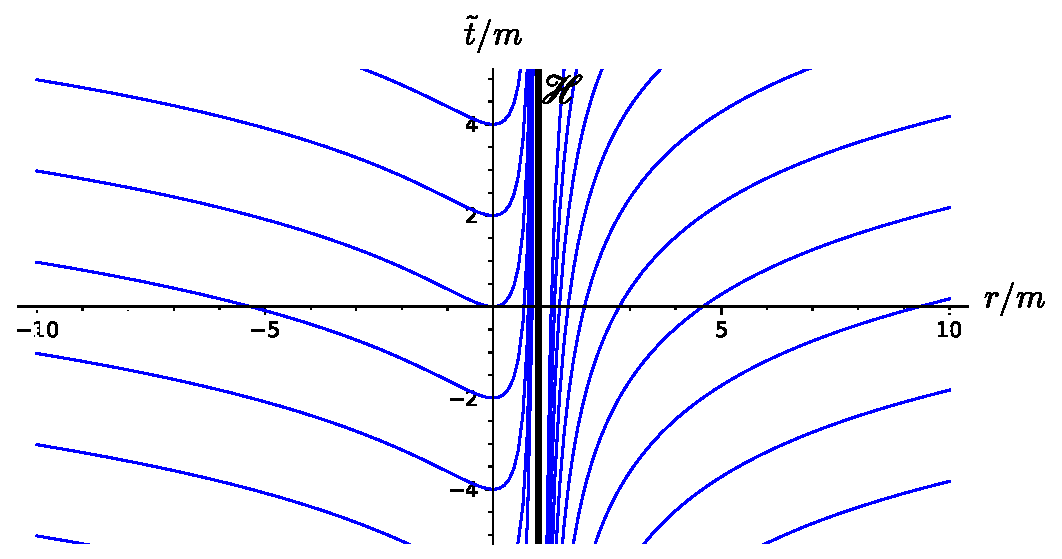
\includegraphics[width=0.7\textwidth]{exk_BL_slicing.pdf}}
\caption[]{\label{f:exk:BL_slicing} \footnotesize
Trace of the hypersurfaces of constant Boyer-Lindquist time $t$ in the plane
$(\tilde{t}, r)$.
\textsl{[Figure generated by the notebook \ref{s:sam:Kerr_extremal}]}
}
\end{figure}

The metric components $(g_{\alpha\beta})$ with respect to the Boyer-Lindquist coordinates $(x^\alpha) = (t,r,\th,\ph)$ are given by
\be \label{e:exk:metric_BL}
    \encadre{
    \begin{array}{ll}
    g_{\mu\nu}\,  \D x^\mu \D x^\nu  = &
    \displaystyle - \left( 1 - \frac{2m r}{\rho^2} \right) \, \D t^2
    - \frac{4 m^2  r \sin^2\th}{\rho^2} \,  \D t\, \D\ph
    + \frac{\rho^2}{(r-m)^2} \, \D r^2  \\[2ex]
    & \displaystyle + \rho^2 \D \th^2
    + \left( r^2 + m^2 + \frac{2 m^3 r \sin^2\th}{\rho^2} \right)
    \sin^2\th \, \D \ph^2 .
    \end{array}
    }
\ee
This expression can be obtained either by taking the limit $a\to m$ of Eq.~(\ref{e:ker:metric_BL})
or by using (\ref{e:exk:dt_dph}) to substitute $\D\ti$ and $\D\tph$ in Eq.~(\ref{e:exk:metric_Kerr_3p1}).
We note that $g_{rr}\to +\infty$ when $r\to m$, which reflects the singularity of Boyer-Lindquist
coordinates on $\Hor$. This singularity is clearly apparent in the coordinate transformations
(\ref{e:exk:3p1_Kerr_to_BL}), as well as in the spacetime slicing by the
hypersurfaces $t=\mathrm{const}$ depicted in Fig.~\ref{f:exk:BL_slicing}: the slices accumulate
onto $\Hor$, without crossing it, so that the points on $\Hor$ do not belong to any
hypersurface $t=\mathrm{const}$. That the $t=\mathrm{const}$ hypersurfaces do not provide a
regular slicing of the extremal Kerr spacetime $(\M,\w{g})$ is also manifest on
the Carter-Penrose diagram shown in Fig.~\ref{f:exk:CPdiag_BL}.

The inverse metric $\w{g}^{-1}$ has the following components in the Boyer-Lindquist coordinates
(cf. the $a\to m$ limit of Eq.~(\ref{e:ker:inv_met_BL})):
\be \label{e:exk:inv_met_BL}
    g^{\alpha\beta} = \left(
    \begin{array}{cccc}
    - \frac{1}{(r-m)^2}
    \left( r^2 + m^2 + \frac{2 m^3 r \sin^2\th}{\rho^2} \right)
     & 0 & 0 & -\frac{2 m^2 r}{\rho^2 (r-m)^2} \\[1ex]
    0 & \frac{(r-m)^2}{\rho^2} & 0 & 0 \\[1ex]
    0 & 0 &\frac{1}{\rho^2} & 0 \\[1ex]
    -\frac{2 m^2 r}{\rho^2 (r-m)^2} & 0 & 0 &
    \frac{1}{(r-m)^2\sin^2\th}\left(1 - \frac{2 m r}{\rho^2} \right)
    \end{array}
    \right) .
\ee

\subsection{Symetries}

The extremal Kerr metric (\ref{e:exk:metric_Kerr_3p1}) is stationary\footnote{Cf.
Sec.~\ref{s:sta:def_station} for the definition of \emph{stationary} and a discussion
about the terminology.} and axisymmetric. The corresponding isometry group is $\R\times\mathrm{SO}(2)$ and is generated
by two commuting Killing vectors $\w{\xi}$ and $\w{\eta}$. Both the Kerr coordinates and
the Boyer-Lindquist ones are adapted to the spacetime symmetries, i.e. $(\ti,\tph)$ and
$(t,\ph)$ are ignorable coordinates, as it is clear on the line elements (\ref{e:exk:metric_Kerr_3p1})
and (\ref{e:exk:metric_BL}). Accordingly, one can normalize the Killing vectors so that
\be
    \encadre{\w{\xi} = \wpar_{\ti} = \wpar_t}
    \qand
    \encadre{\w{\eta} = \wpar_{\tph} = \wpar_\ph} .
\ee

\begin{figure}
\centerline{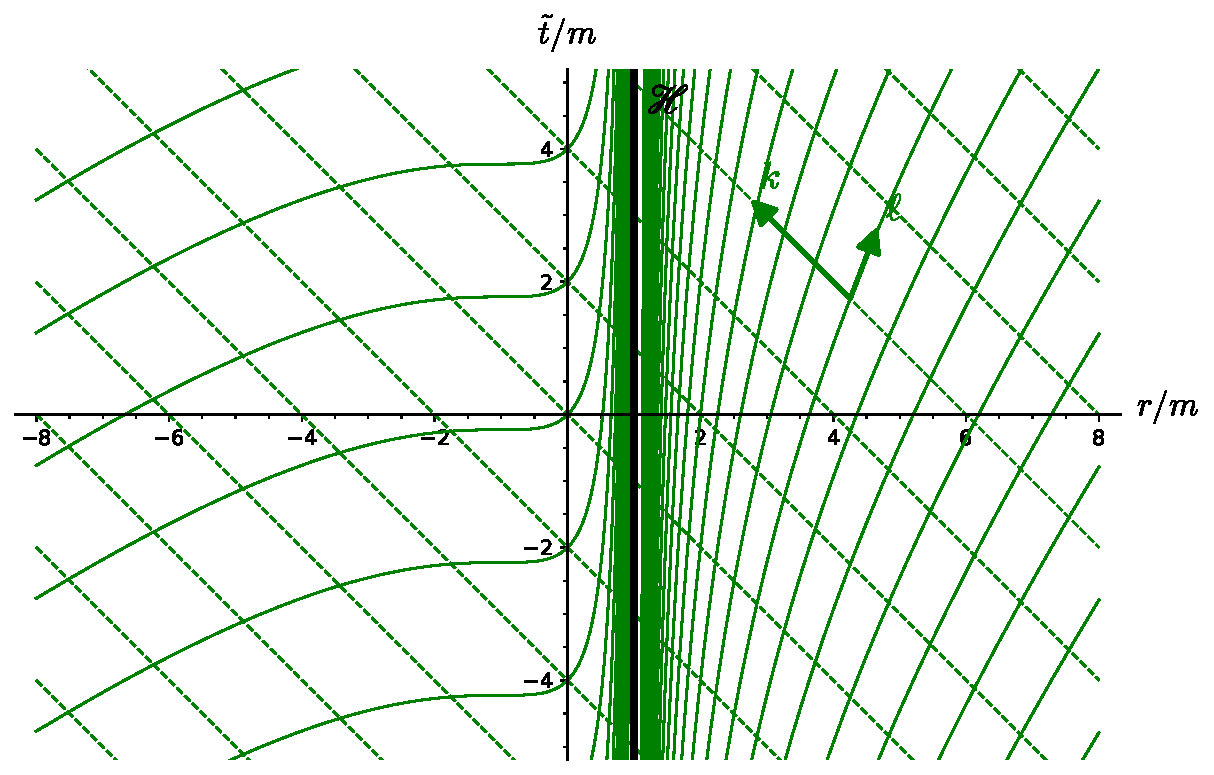
\includegraphics[width=0.8\textwidth]{exk_princ_null_geod.pdf}}
\caption[]{\label{f:exk:princ_null_geod} \footnotesize
Trace of the principal null geodesics in the plane
$(\tilde{t}, r)$. The dashed lines correspond to the
ingoing principal null geodesics $\Li^{\rm in}_{(v,\th,\tph)}$
and the solid curves to the
outgoing principal null geodesics $\Li^{\rm out,I}_{(u,\th,\tilde{\tph})}$
for $r>m$ and $\Li^{\rm out,III}_{(u,\th,\tilde{\tph})}$ for $r<m$.
\textsl{[Figure generated by the notebook \ref{s:sam:Kerr_extremal}]}
}
\end{figure}



\subsection{Principal null geodesics} \label{s:exk:princ_null_geod}

As discussed in Sec.~\ref{s:ker:principal_geod}, the Kerr spacetime is
endowed with two congruences of null geodesics that are tied to
the spacetime structure, as described by the Weyl conformal curvature tensor.
All the results of Sec.~\ref{s:ker:principal_geod} remain valid at the limit $a\to m$.
We can summarize them as follows:
\begin{greybox}
\begin{itemize}
\item The \defin{ingoing principal null geodesics} are the curves
\be
    \Li^{\rm in}_{(v,\th,\tph)}:\quad
        (v,\th,\tph) = \mathrm{const} \in \R\times[0,\pi]\times[0,2\pi), %]
\ee
where $v$ is the Kerr advanced time:
\be \label{e:exk:def_v}
    v := \ti + r = t  + r - \frac{2m^2}{r -m} + 2m\ln\left| \frac{r - m}{m} \right|.
\ee
Along the geodesic $\Li^{\rm in}_{(v,\th,\tph)}$, $-r$ is an affine parameter increasing towards the future;
the corresponding tangent vector is
\begin{subequations}
\begin{align}
 \w{k} & = \wpar_{\ti} - \wpar_{\tilde{r}} \label{e:exk:k_3p1_Kerr}\\
 \w{k} & = \frac{r^2 + m^2}{(r - m)^2} \, \wpar_t
            - \wpar_r + \frac{m}{(r - m)^2} \, \wpar_\ph
            \quad \mbox{in}\ \M\setminus\Hor .  \label{e:exk:k_BL}
\end{align}
\end{subequations}
\item The \defin{outgoing principal null geodesics} are the curves
\begin{subequations}
\begin{align}
  \mbox{in}\ \M_{\rm I} :&\quad \Li^{\rm out, I}_{(u,\th,\tilde{\tph})}:
    \quad   (u,\th,\tilde{\tph}) = \mathrm{const} \in \R\times[0,\pi]\times[0,2\pi), \\ %]
  \mbox{in}\ \M_{\rm III}:&\quad \Li^{\rm out, III}_{(u,\th,\tilde{\tph})}:
    \quad   (u,\th,\tilde{\tph}) = \mathrm{const} \in \R\times[0,\pi]\times[0,2\pi), \\ %]
 \mbox{on}\  \Hor: &\quad \Li^{{\rm out},\Hor}_{(\th,\psi)}:
    \quad  (\th,\psi) = \mathrm{const} \in [0,\pi]\times[0,2\pi),  %]
\end{align}
\end{subequations}
where $u$ is the Kerr retarded time:
\be \label{e:exk:def_u}
    u := \ti - r + \frac{4 m^2}{r - m} - 4 m \ln \left| \frac{r - m}{m} \right|
      = t  - r + \frac{2m^2}{r -m} - 2m\ln\left| \frac{r - m}{m} \right| ,
\ee
\be \label{e:exk:def_ttph}
    \tilde{\tph} := \tph + \frac{2m}{r -m} = \ph + \frac{m}{r - m}
\ee
and
\be \label{e:exk:psi_tph_ti}
    \psi := \tph - \frac{\ti}{2m} .
\ee
Along the geodesics $\Li^{\rm out, I}_{(u,\th,\tilde{\tph})}$ and $\Li^{\rm out, III}_{(u,\th,\tilde{\tph})}$,
$r$ is an affine parameter increasing towards the future,
while along $\Li^{{\rm out},\Hor}_{(\th,\psi)}$, such an affine parameter is $\ti$. The null tangent vector $\wl$ along the outgoing principal null geodesics
that coincides with the Killing vector $\w{\xi} + (2m)^{-1} \w{\eta}$ on $\Hor$ is
\begin{subequations}
\begin{align}
 \wl & = \frac{(r + m)^2}{2(r^2 + m^2)}\, \wpar_{\ti}
  + \frac{(r - m)^2}{2(r^2 + m^2)} \,  \wpar_{\tilde{r}}
  + \frac{m}{r^2 + m^2} \, \wpar_{\tph} \label{e:exk:ell_3p1_Kerr}\\
 \wl & =  \frac{1}{2}\, \wpar_t
            + \frac{(r - m)^2}{2(r^2 + m^2)} \,  \wpar_r
            + \frac{m}{2(r^2 + m^2)} \, \wpar_\ph
            \quad \mbox{in}\ \M\setminus\Hor . \label{e:exk:ell_BL}
\end{align}
\end{subequations}
\end{itemize}
\end{greybox}
\begin{proof}
The second equality in Eq.~(\ref{e:exk:def_v}) follows from Eq.~(\ref{e:exk:3p1_Kerr_to_BL_t}).
Eq.~(\ref{e:exk:k_BL}) follow from Eq.~(\ref{e:exk:k_3p1_Kerr}) via Eq.~(\ref{e:exk:frame_BL_Kerr3p1}).
Eqs.~(\ref{e:exk:def_u}) and (\ref{e:exk:def_ttph}) are the integrated version of the system (\ref{e:ker:out_Kerr_Kerr_3p1}) with $a=m$. Equations~(\ref{e:exk:psi_tph_ti}), (\ref{e:exk:ell_3p1_Kerr})
and (\ref{e:exk:ell_BL}) are the $a=m$ versions of respectively
Eqs.~(\ref{e:ker:psi_tph_ti}), (\ref{e:ker:def_ell_outgoing}) and (\ref{e:ker:ell_BL}).
All the other statements follow from the $a\to m$ limit of results of Sec.~\ref{s:ker:principal_geod},
except for $\ti$ being an affine parameter along $\Li^{{\rm out},\Hor}_{(\th,\psi)}$, which
is peculiar to the extremal Kerr horizon and will
be proven in Sec.~\ref{s:exk:horizon}.
\end{proof}

The principal null geodesic congruences are depicted in terms of the $(\ti, r)$
coordinates in Fig.~\ref{f:exk:princ_null_geod}. Note that the outgoing geodesics
$\Li^{\rm out, I}_{(u,\th,\tilde{\tph})}$ and $\Li^{\rm out, III}_{(u,\th,\tilde{\tph})}$
tend to become tangent to $\Hor$ for $r\to m$; this agrees with $\Hor$ being
generated by some members of the outgoing principal null congruence, namely the geodesics
$\Li^{{\rm out},\Hor}_{(\th,\psi)}$, as we shall see in details in the next subsection.
Another view of the principal null geodesics is provided by the Carter-Penrose
diagram of $(\M,\w{g})$ shown in Fig.~\ref{f:exk:CPdiag_Kerr}.

\subsection{The degenerate horizon} \label{s:exk:horizon}

$\Hor$ is the hypersurface of $\M$ defined by $r=m$ [Eq.~(\ref{e:exk:def_H})]. Given
that the component $g^{rr} = (r - m)^2/\rho^2$ of the inverse metric with respect to Kerr coordinates vanishes at $r=m$ [cf. Eq.~(\ref{e:exk:inv_met_3p1})], we have
$g^{\tilde{\mu}\tilde{\nu}} \partial_{\tilde{\mu}} r \partial_{\tilde{\nu}} r = 0$ on $\Hor$,
which implies that the gradient $\vw{\nabla} r$
is a null vector there and that $\Hor$ is a null hypersurface.
Moreover, since the components of $\vw{\nabla} r$ are $\nabla^{\tilde{\alpha}} = g^{\tilde{\alpha}r}$,
we read on Eq.~(\ref{e:exk:inv_met_3p1}) that
\be
    \vw{\nabla} r \equalH \frac{2m^2}{\rho^2} \wpar_{\ti} + \frac{m}{\rho^2} \wpar_{\tph}
        \equalH \frac{2 m^2}{\rho^2} \w{\chi} ,
\ee
where $\w{\chi}$ is the Killing vector field
\be \label{e:exk:def_chi}
    \w{\chi} := \w{\xi} + \Omega_H \w{\eta} , \qquad\mbox{with}\quad \Omega_H := \frac{1}{2m} .
\ee
It follows immediately that $\Hor$ is a \emph{Killing horizon}, i.e. a null hypersurface
that admits a Killing vector as null normal (cf. the definition given in
Sec.~\ref{s:neh:def_Killing_hor}).

From expression~(\ref{e:exk:ell_3p1_Kerr}) for $\wl$, we have immediately
\be \label{e:exk:ell_chi_on_H}
    \wl \equalH \w{\chi} .
\ee
This means that the null generators of $\Hor$ are the outgoing principal null
geodesics $\Li^{{\rm out},\Hor}_{(\th,\psi)}$.

The \emph{surface gravity}\index{surface!gravity} $\kappa$ of the Killing horizon $\Hor$
has been defined in Sec.~\ref{s:neh:zeroth_law} as the non-affinity coefficient of the Killing-vector normal $\w{\chi}$ to $\Hor$:
$\wnab_{\w{\chi}}\, \w{\chi} \equalH \kappa \, \w{\chi}$ [cf. Eq.~(\ref{e:neh:xi_nab_xi_kappa})].
Given identity (\ref{e:exk:ell_chi_on_H}), $\kappa$ coincides with the value on $\Hor$ of the
non-affinity coefficient $\kappa_{\wl}$ of the tangent $\wl$ to the outgoing principal null
geodesics: $\wnab_{\wl}\, \wl = \kappa_{\wl}\, \wl$. A direct computation (cf. the notebook~\ref{s:sam:Kerr_extremal}) reveals that
\be
    \kappa_{\wl} = m \frac{r^2 - m^2}{(r^2 + m^2)^2} .
\ee
In particular, $\kappa_{\wl}$ vanishes for $r=m$, i.e. on $\Hor$.
Since $\kappa = \left. \kappa_{\wl} \right| _{\Hor}$, we
get\footnote{The vanishing of $\kappa$ can also be obtained
by taking the limit $a\to m$ of expression (\ref{e:ker:kappa_m_a}) derived for $a<m$.}
\be
    \encadre{\kappa = 0 } .
\ee
According to the classification introduced in Sec.~\ref{s:neh:classif_KH}, one says
that $\Hor$ is a \emph{degenerate Killing horizon}\index{degenerate!Killing horizon}\index{Killing!horizon!degenerate --}.
The vanishing of the non-affinity parameter $\kappa$ means that $\wl$ is a geodesic vector\index{geodesic!vector}
on $\Hor$, and not only a pregeodesic\index{pregeodesic!vector field}  one (cf. Remark~\ref{r:fra:geodesic_vector} in Sec.~\ref{s:fra:geod_motion}). Equivalently, at any given point $p\in\Hor$,
$\wl$ is the tangent vector associated to
an affine parameter $\lambda$ of the null geodesic $\Li^{{\rm out},\Hor}_{(\th,\psi)}$ through $p$.
Moreover, the affine parameter $\lambda$ coincides with $\ti$,
up to some additive constant. Indeed,
Eq.~(\ref{e:exk:ell_chi_on_H}) implies
\[
     \ell^{\ti} = \derd{\ti}{\lambda} = \chi^{\ti} = 1 ,
\]
from which $\lambda = \ti + \mathrm{const}$.
Since the range of $\ti$ is $(-\infty, +\infty)$, we conclude that
$\Li^{{\rm out},\Hor}_{(\th,\psi)}$ is a complete geodesic. This constrasts
with the null generators of a non-degenerate Killing horizon, which are
incomplete, as shown in Sec.~\ref{s:sta:non-degenerate_KH}.

Let us summarize the results obtained above:
\begin{greybox}
In the extremal Kerr spacetime, the hypersurface $\Hor$ defined
by $r=m$ is a degenerate Killing horizon.
Its generators are the outgoing principal null geodesics
$\Li^{{\rm out},\Hor}_{(\th,\psi)}$, which are complete geodesics
and which admit $\ti$ as an affine parameter. The tangent vector associated to this affine
parameter is the Killing vector $\w{\chi} = \w{\xi} + \Omega_H \w{\eta}$
[Eq.~(\ref{e:exk:def_chi})], which coincides on $\Hor$ with the tangent
vector $\wl$ to the outgoing principal null congruence.
\end{greybox}

\subsection{Black hole character}

As a Killing horizon, $\Hor$ is a null hypersurface and thus a one-way membrane.
Since the ingoing principal null geodesics $\Li^{\rm in}_{(v,\th,\tph)}$
cross it from $\M_{\rm I}$ to $\M_{\rm III}$ (cf. Fig.~\ref{f:exk:princ_null_geod}),
we conclude that no (massive or null) particle can cross $\Hor$ from $\M_{\rm III}$
to $\M_{\rm I}$.
In order to show that $\Hor$ is actually a black hole event horizon,
it suffices to proceed as for the $a<m$ case treated in Sec.~\ref{s:ker:event_hor}.
We shall not repeat the argument here (which is based on the
asymptotics of Kerr spacetime being that of Schwarzschild spacetime --- a property
that holds for the extremal Kerr spacetime as well) and jump directly to the conclusion:
\begin{greybox}
The extremal Kerr spacetime $(\M, \w{g})$ can be endowed with a conformal
completion at null infinity such that the future null infinity $\scri^+$
is located at the boundary of $\M_{\rm I}$. The region $\M_{\rm III}$ is
then the interior of a black hole, the event horizon of which is
the Killing horizon $\Hor$.
\end{greybox}

The future null infinity $\scri^+$ and the past null infinity $\scri^-$
relative to $\M_{\rm I}$ are depicted in the Carter-Penrose diagram of
Figs.~\ref{f:exk:CPdiag_Kerr} -\ref{f:exk:CPdiag_BL}. In this diagram,
it is clear that $\M_{\rm III}$ is a black hole region for $\M_{\rm I}$
and that $\Hor$ is the corresponding event horizon.

\begin{figure}
\centerline{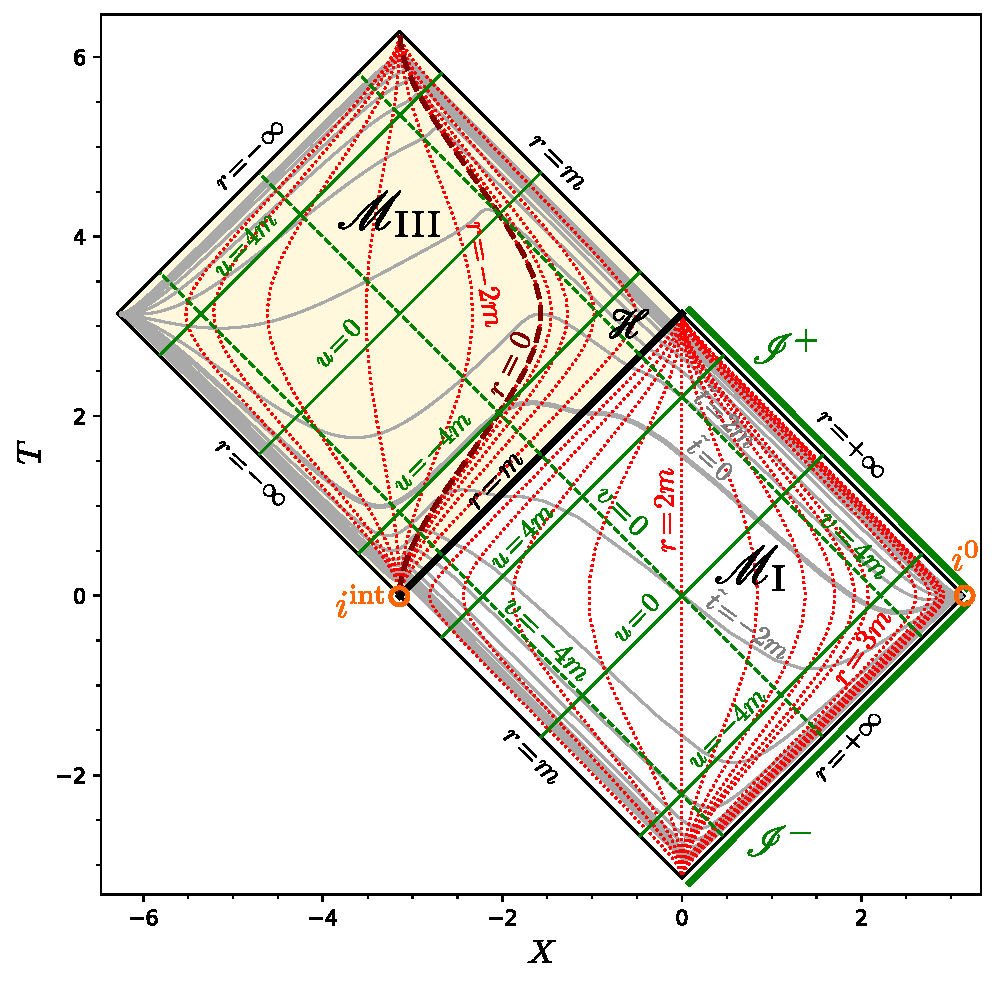
\includegraphics[width=0.8\textwidth]{exk_CPdiag_Kerr.pdf}}
\caption[]{\label{f:exk:CPdiag_Kerr} \footnotesize
Carter-Penrose diagram of the extremal Kerr spacetime $(\M,\w{g})$,
with the time slicing associated to the Kerr coordinates $(\ti, r,\th,\tph)$.
The Carter-Penrose diagram (cf. Sec.~\ref{s:ker:Carter_Penrose_diag})
is constructed via the projection
map $\Pi:\ \M \to \R^2$,  $(\ti,r,\th,\tph)\mapsto (T, X)$
defined by $T = T_0(\ti, r) := \arctan(u/2) + \arctan(v/2)$,
$X = X_0(\ti, r) := \arctan(v/2) - \arctan(u/2)$ for $r>m$
and $T = T_0(\ti, r) + \pi$, $X = X_0(\ti, r) - \pi$ for $r<m$,
where $u$ and $v$ are the functions of $(\ti, r)$ given by
Eqs.~(\ref{e:exk:def_u}) and (\ref{e:exk:def_v}) respectively.
The grey curves represent hypersurfaces $\ti=\mathrm{const}$, with
$\ti\in[-20 m, 20 m]$ and
the increment $\delta\ti = 2 m$ between two successive hypersurfaces.
The hypersurface $\ti=0$ is singled out by a larger thickness.
The red dotted curves represent hypersurfaces $r=\mathrm{const}$,
with the increment $\delta r$ between two successive hypersurfaces being
$\delta r = 2m$ for $r<0$ and $r> 3m$ and $\delta r = 0.2\, m$ for $0\leq r \leq 3m$.
The hypersurface $r=0$ is marked by the brown dashed line.
The green straight lines depict some selected principal null geodesics
(dashed = ingoing, solid = outgoing, as in Fig.~\ref{f:exk:princ_null_geod}).
\textsl{[Figure generated by the notebook \ref{s:sam:Kerr_extremal}]}
}
\end{figure}


\begin{figure}
\centerline{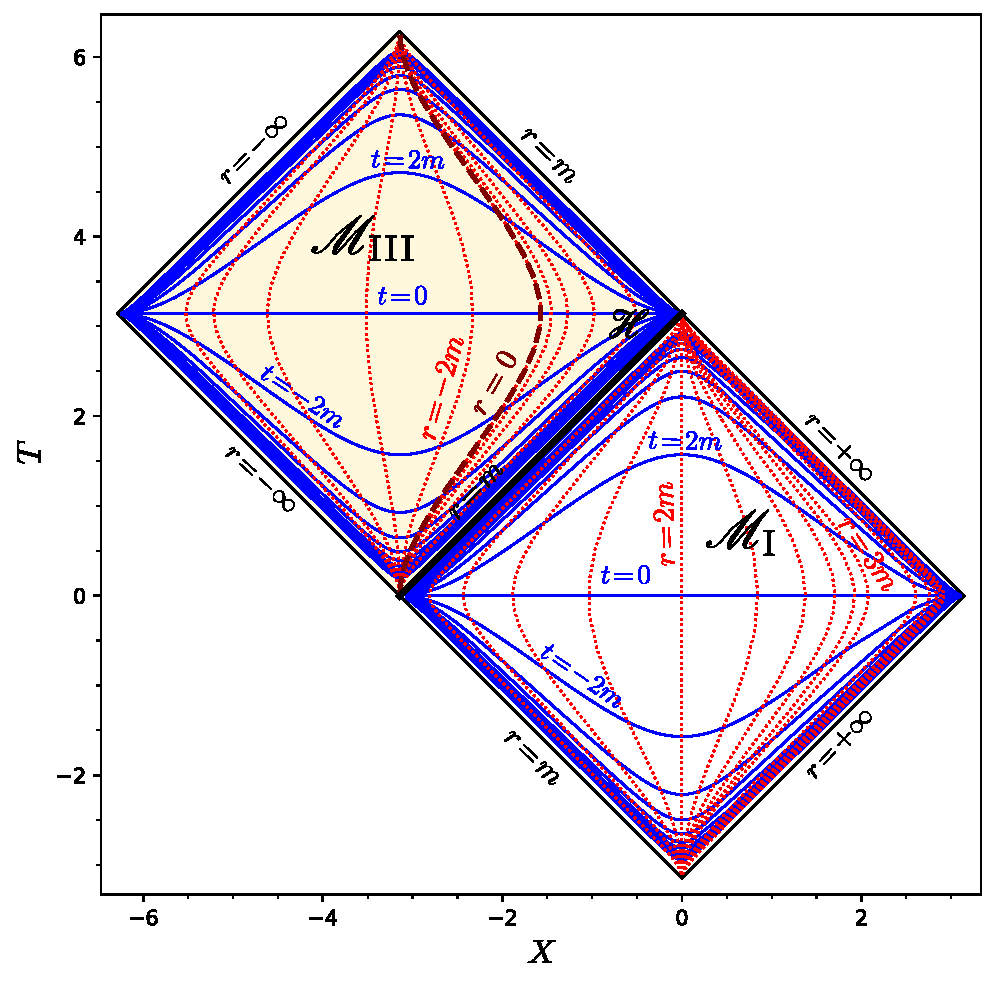
\includegraphics[width=0.8\textwidth]{exk_CPdiag_BL.pdf}}
\caption[]{\label{f:exk:CPdiag_BL} \footnotesize
Same as Fig.~\ref{f:exk:CPdiag_Kerr} but for the
time slicing associated to Boyer-Lindquist coordinates $(t,r,\th,\ph)$.
The blue curves represent hypersurfaces $t=\mathrm{const}$, with
$t\in[-20 m, 20 m]$ and
the increment $\delta t = 2 m$ between two successive hypersurfaces.
Note that the spacetime slicing by the hypersurfaces $t=\mathrm{const}$
is singular at $\Hor$, contrary to the slicing by the hypersurfaces
of constant Kerr time $\ti$ shown in Fig.~\ref{f:exk:CPdiag_Kerr}.
\textsl{[Figure generated by the notebook \ref{s:sam:Kerr_extremal}]}
}
\end{figure}

%%%%%%%%%%%%%%%%%%%%%%%%%%%%%%%%%%%%%%%%%%%%%%%%%%%%%%%%%%%%%%%%%%%%%%%%%%%%%%%

\section{Maximal analytic extension}

\subsection{Extension of $\M_{\rm I}$ for complete outgoing principal null geodesics}

Figure~\ref{f:exk:CPdiag_Kerr} presents a Carter-Penrose diagram\footnote{Cf. Sec.~\ref{s:ker:Carter_Penrose_diag} for the definition of such a diagram.} of
the extremal Kerr spacetime $(\M,\w{g})$ with some outgoing principal null geodesics
$\Li^{\rm out, I}_{(u,\th,\tilde{\tph})}$ and $\Li^{\rm out, III}_{(u,\th,\tilde{\tph})}$
plotted for some selected values of $u$ (green solid lines).
Let us consider the ``external'' region $\M_{\rm I}$.
Since $r$ is an affine parameter along the null geodesics $\Li^{\rm out, I}_{(u,\th,\tilde{\tph})}$,
it is clear that these geodesics are incomplete, for they all terminate
in the past at the finite value $r=m$ (the South-West boundary
of $\M_{\rm I}$ in Fig.~\ref{s:ker:Carter_Penrose_diag}), without any possible
extension into $\M_{\rm III}$ from there.
To extend $\M_{\rm I}$ so that all geodesics $\Li^{\rm out, I}_{(u,\th,\tilde{\tph})}$
are complete, let us introduce a coordinate system on $\M_{\rm I}$ that is
adapted to the outgoing principal null geodesics, as the Kerr coordinates
$(\ti,r,\th,\tph)$ were adapted to the ingoing ones.
We thus define the \defin{outgoing Kerr coordinates}\index{outgoing!Kerr coordinates}\index{Kerr!coordinates!outgoing --} $(x^{\tilde{\tilde\alpha}})=(\tilde{\ti},r,\th,\tilde{\tph})$ by
\be \label{e:exk:ttt_u}
    u = \tilde{\ti} - r \iff \tilde{\ti} = u + r  ,
\ee
where $u$ is the retarded Kerr time (\ref{e:exk:def_u}) and $\tilde{\tph}$
is related to the angle $\tph$ of Kerr coordinates or to the angle
$\ph$ of Boyer-Lindquist coordinates by Eq.~(\ref{e:exk:def_ttph}).
By construction, the tangent vector to $\Li^{\rm out, I}_{(u,\th,\tilde{\tph})}$
associated with the affine parameter $r$ is then
\be
    \wl' = \wpar_{\tilde{\ti}} + \wpar_{\tilde{\tilde{r}}},
\ee
where $\wpar_{\tilde{\tilde{r}}}$ stands for the vector $\partial/\partial r$
of the coordinates $(\tilde{\ti},r,\th,\tilde{\tph})$.
Indeed ${\ell'}^{\tilde{\tilde\alpha}} = \D x^{\tilde{\tilde\alpha}} /\D r
= (1, 1, 0, 0)$ since along $\Li^{\rm out, I}_{(u,\th,\tilde{\tph})}$,
$\tilde{\ti} = r + u$, with $u$ constant, and both $\th$ and $\tilde{\tph}$
are constant. An explicit computation (cf. the notebook ??) shows that
$\wl'$ is a geodesic vector:
\be
    \wnab_{\wl'} \wl' = 0 ,
\ee
which confirms that $r$ is an affine parameter along $\Li^{\rm out, I}_{(u,\th,\tilde{\tph})}$.
$\wl'$ is thus similar to $\w{k}$, which is
the tangent vector to the ingoing principal null geodesics $\Li^{\rm in}_{(v,\th,\tph)}$
associated with the affine parameter $-r$ along them.
In this respect, note the symmetry between the relations
$\wl' = \wpar_{\tilde{\ti}} + \wpar_{\tilde{\tilde{r}}}$
and $\w{k} = \wpar_{\ti} - \wpar_{\tilde{r}}$ [Eq.~(\ref{e:exk:k_3p1_Kerr})].
The link between $\wl'$ and the tangent vector $\wl$ to $\Li^{\rm out, I}_{(u,\th,\tilde{\tph})}$
introduced in Sec.~\ref{s:exk:princ_null_geod} is easily obtained from
the definition of a tangent vector to a curve:
\[
    \wl' = \frac{\D\w{x}}{\D r} = \frac{\D\w{x}}{\D\lambda} \frac{\D\lambda}{\D r}
        = \left(\frac{\D r}{\D \lambda} \right) ^{-1} \wl ,
\]
where $\lambda$ is the (non-affine) parameter of $\Li^{\rm out, I}_{(u,\th,\tilde{\tph})}$
associated with $\wl$. We read on the Kerr components (\ref{e:exk:ell_3p1_Kerr})
of $\wl$, as well as on the Boyer-Lindquist ones (\ref{e:exk:ell_BL}), that
$\D r/\D\lambda = \ell^r = (r-m)^2/(2(r^2 + m^2))$. Hence
\be
    \wl' = 2 \frac{r^2 + m^2}{(r - m)^2} \, \wl .
\ee

Substituting Eq.~(\ref{e:exk:def_u}) for $u$ into $\tilde{\ti} = u + r$
[Eq.~(\ref{e:exk:ttt_u})], we get the expression of $\tilde{\ti}$ in terms of the
Kerr time $\ti$ and the Boyer-Lindquist time $t$:
\be \label{e:exk:ttt_t_ti}
    \tilde{\ti} = \ti + \frac{4 m^2}{r - m} - 4 m \ln \left| \frac{r - m}{m} \right|
      = t + \frac{2m^2}{r -m} - 2m\ln\left| \frac{r - m}{m} \right| .
\ee
This relation is to be supplemented by Eq.~(\ref{e:exk:def_ttph}) to fully
specify the transformation from respectively the Kerr coordinates
$(\ti,r,\th,\tph)$ and the Boyer-Lindquist coordinates
$(t,r,\th,\ph)$ to the outgoing Kerr coordinates
$(\tilde{\ti},r,\th,\tilde{\tph})$.
Differentiating Eqs.~(\ref{e:exk:ttt_t_ti}) and (\ref{e:exk:def_ttph})
leads to
\be \label{e:exk:Dttt_Dtph_Kerr}
    \D\tilde{\ti} = \D\ti - \frac{4 m r}{(r-m)^2} \D r
    \qand
    \D\tilde{\tph} = \D\tph - \frac{2 m}{(r-m)^2} \D r
\ee
and
\be \label{e:exk:Dttt_Dtph_BL}
    \D\tilde{\ti} = \D t - \frac{2 m r}{(r-m)^2} \D r
    \qand
    \D\tilde{\tph} = \D\ph - \frac{m}{(r-m)^2} \D r
\ee

\begin{remark}
Equation~(\ref{e:exk:Dttt_Dtph_BL}) differs from
Eq.~(\ref{e:exk:dt_dph}) only by the sign $+$ changed to $-$ in the
right-hand side. This reflects the complete symmetry between the Kerr coordinates
$(\ti,r,\th,\tph)$
and the outgoing Kerr coordinates
$(\tilde{\ti},r,\th,\tilde{\tph})$
from the point of view of the Boyer-Lindquist coordinates $(t,r,\th,\ph)$
(cf. the discussion at the beginning of Sec.~\ref{s:ker:out_princ_null_geod}).
\end{remark}

From Eq.~(\ref{e:exk:Dttt_Dtph_Kerr}) and the chain rule, we get immediately
the link between the outgoing Kerr coordinate frame and the Kerr coordinate frame:
\be
    \wpar_{\tilde{\ti}} = \wpar_{\ti},\qquad
    \wpar_{\tilde{\tilde{r}}} = \wpar_{\tilde{r}} + \frac{4 m r}{(r-m)^2} \wpar_{\ti}
        + \frac{2m}{(r-m)^2} \wpar_{\tph}, \qquad
    \wpar_{\th} = \wpar_{\th},\qquad
    \wpar_{\tilde{\tph}} = \wpar_{\tph} .
\ee

The components of the metric tensor with respect to the
outgoing Kerr coordinates are easily obtained by substituting $\D t$ and $\D\ph$
from Eq.~(\ref{e:exk:Dttt_Dtph_BL}) into the Boyer-Lindquist expression
(\ref{e:exk:metric_BL}) (see also the notebook~??); we get
\be
    \begin{array}{ll}
    g_{\tilde{\tilde{\mu}}\tilde{\tilde{\nu}}}\, \D x^{\tilde{\tilde{\mu}}} \, \D x^{\tilde{\tilde{\nu}}}   = &
    \displaystyle - \left( 1 - \frac{2m r}{\rho^2} \right)  {\D\tilde{\ti}}^2
    - \frac{4m r}{\rho^2} \D\tilde{\ti}\, \D r
    - \frac{4 m^2  r \sin^2\th}{\rho^2} \,  \D\tilde{\ti}\, \D\tilde{\tph} \\[2ex]
    &\displaystyle  + \left( 1 + \frac{2m r}{\rho^2} \right) \D r^2
     + 2 m \left( 1 + \frac{2m r}{\rho^2} \right) \sin^2\th \, \D r\, \D\tilde{\tph} \\[2ex]
    & \displaystyle + \rho^2 \D \th^2
    + \left( r^2 + m^2 + \frac{2 m^3 r \sin^2\th}{\rho^2} \right)
    \sin^2\th \, {\D\tilde{\tph}}^2 .
    \end{array}
\ee



\section{Near-horizon extremal Kerr metric}

\subsection{The extremal Kerr throat}















